\documentclass[../manuale_sviluppatore.tex]{subfiles}

\begin{document}

\subsection{Design Pattern architetturale: MVP}
Il design pattern architetturale scelto per il prodotto è il \glossario{Model View Presenter}. 
Di conseguenza le componenti principali del prodotto sono le seguenti:
\begin{itemize}
	\item \textbf{Model}: tra i model figurano tutti i tipi che hanno il compito di mantenere i dati 
	del dominio, nello specifico vi sono il dataset, la matrice delle distanze e i modelli delle visualizzazioni 
	che preservano la configurazione delle stesse;
	\item \textbf{Presenter}: tra i presenter figurano tutti i tipi che implementano la logica di 
	business e la logica di visualizzazione, in particolare vi sono i presenter delle visualizzazioni, 
	degli elementi di modifica dei grafici e i manager dell'applicazione che ne gestiscono il corretto funzionamento;
	\item \textbf{View}: le view sono dei tipi sostanzialmente passivi che visualizzano i dati di dominio 
	secondo la configurazione dell'applicazione, ed indirizzano gli eventi ai presenter affinchè essi 
	li elaborino e producano degli aggiornamenti coerenti con li stessi; tra le view vi sono il 
	codice HTML dei grafici e i diversi tipi degli elementi di modifica dei grafici.

\end{itemize}
Nella nostra architettura le componenti (elementi per la modifica delle proprietà dei grafici) 
dispongono ciascuno di un presenter e di una view, non hanno un loro modello specifico in quanto i 
loro dati dipendono dal modello dei grafici, dal dataset o dalla matrice delle distanze. Nel caso dei
grafici invece la view viene realizzata tramite le funzionalità di D3.

\begin{figure}[H]
	\centering
	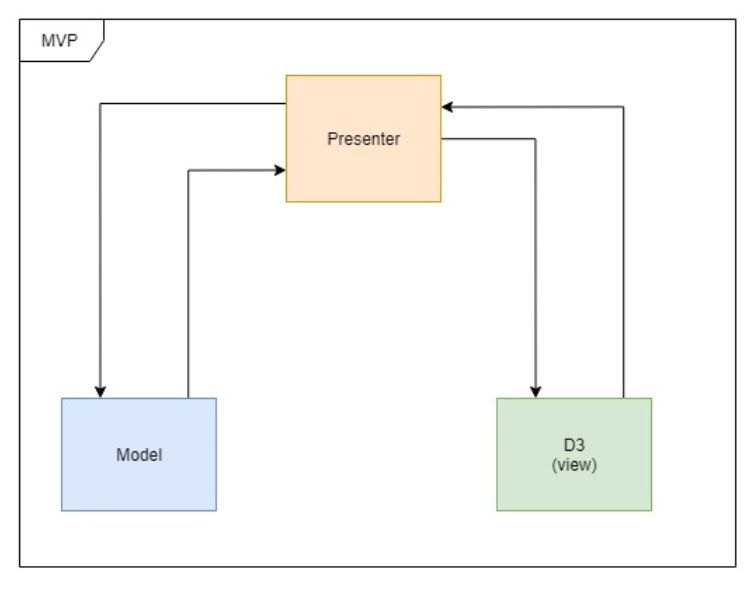
\includegraphics[width=18cm]{img/patternMVP.jpg}
	\caption{Pattern MVP}
\end{figure}

\subsection{Architettura di dettaglio}
\subsubsection{Il client}

Per la definizione dei package del prodotto si è deciso di seguire il principio di progettazione 
\emph{Common Reuse Principle}, di modo da avere tipi che vengono utilizzati assieme all'interno 
dello stesso package.
I package principali sono:
\begin{itemize}
	\item \textbf{Util}: all'interno del package sono presenti tutti i tipi di supporto necessari 
	nell'applicazione, come per esempio l'implementazione del design pattern observer, largamente 
	utilizzata all'interno del prodotto;
	\item \textbf{Core}: all'interno del package vi sono tutti i tipi relativi alle strutture dati 
	cardine del prodotto, ossia il \emph{Dataset} e la \emph{DistanceMatrix}, oltre 
	all'implementazione del design pattern strategy per la scelta della distanza da utilizzare;
	\item \textbf{HD-Viz}: contiene i manager, tipi che realizzano la \emph{dependency inversion} e 
	garantiscono il corretto funzionamento dell'applicazione;
	\item \textbf{Graphs}: package che contiene i tidi dei modelli, dei presenter e le view dei 
	grafici di HD-Viz;
	\item \textbf{Components}: contiene i tipi dei presenters e delle views dei diversi componenti, 
	ossia quegli elementi che si interfacciano con il \emph{Dataset}, la \emph{DistanceMatrix} o i 
	modelli dei grafici e ne modificano i dati o le proprietà di visualizzazione.
\end{itemize}

\begin{figure}[H]
	\centering
	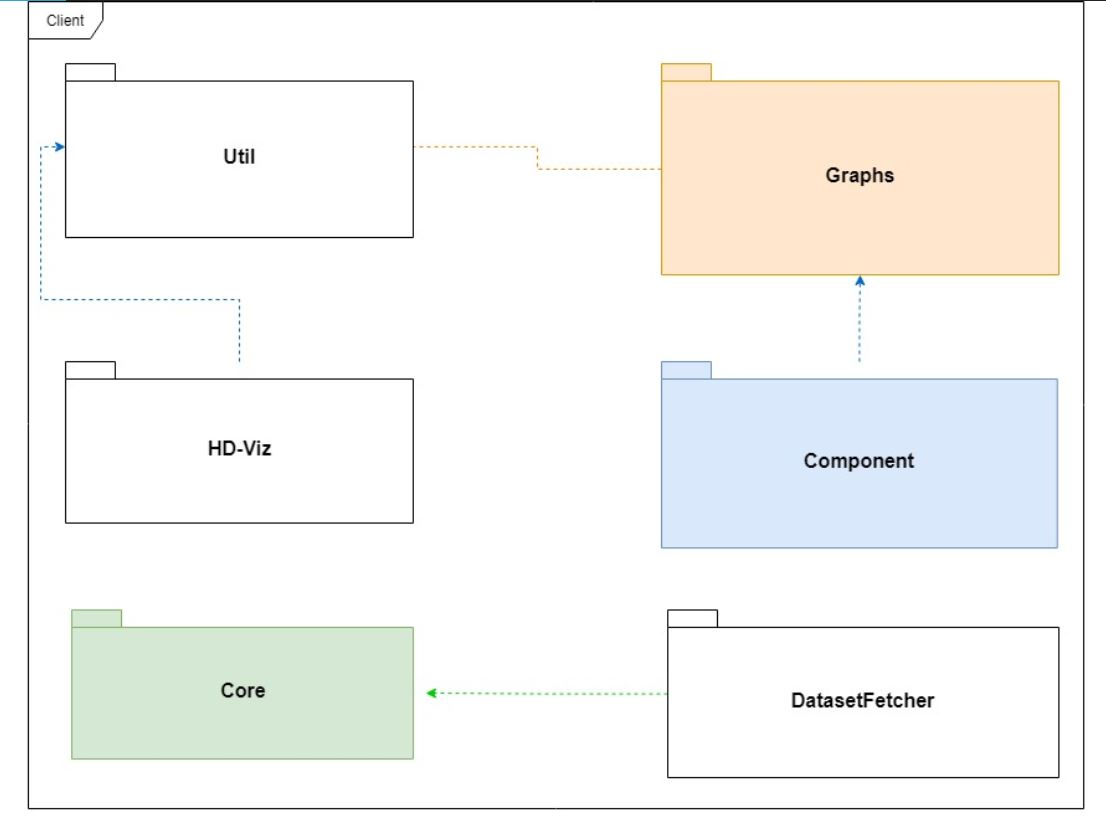
\includegraphics[width=18cm]{img/core.jpg}
	\caption{Struttura generale Hd-Viz}
\end{figure}

\emph{HD Viz manager} è il core dell'architettura, esso implementa la \emph{dependency inversion}, 
infatti si occupa di tener traccia dei dati per evitare istanze multiple del \glossario{Dataset}, 
della \emph{DistanceMatrix} e dei grafici una volta creati. 
Nel momento in cui viene modificato il dataset originale per modificare le visualizzazioni, esso 
funge da tramite creando una copia del dataset e usando quest'ultima per le modifiche, cosicchè il 
dataset originale resti invariato.
\emph{HdVizManager} collabora con diversi altri manager che si occupano di gestire aspetti più 
specifici dell'applicazione, come ad esempio \emph{GraphCreatorManager} che gestisce le factories 
per la creazione dei vari modelli dei grafici. 
Il \emph{CurrentGraphManager} verifica se le factories sono in grado di costruire il grafico, 
quindi si occupa di comunicare con il presenter e il modello del grafico relativo. \\


\begin{figure}[H]
	\centering
	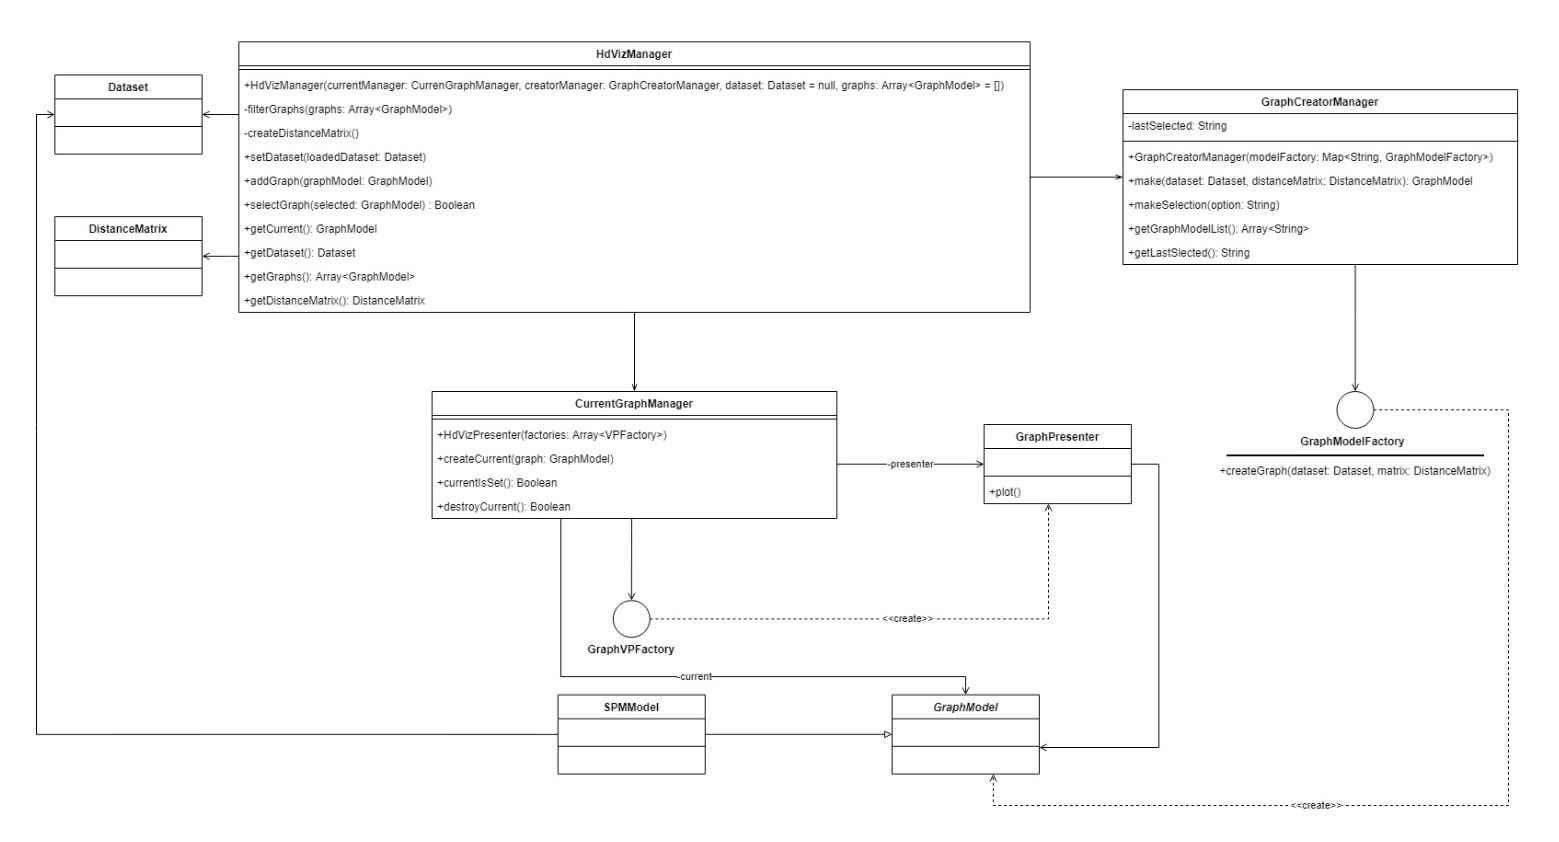
\includegraphics[width=18cm]{img/core-hdvizmanager.jpg}
	\caption{HD-Viz Manager}
\end{figure}

Graphs contiene le diverse visualizzazioni che la nostra applicazione metterà a disposizione, Component mette a disposizione una serie di componenti che permettono di aggiungere funzionalità ai grafici.
Questi ultimi modificano le proprietà di visualizzazione dei grafici, dialogando con modelli tramite interfacce. Ciascun component ha un \emph{Presenter} che gestisce la logica e la \emph{View} che renderizza il tutto,
infatti tramite le interfacce ogni grafico implementerà dimensioni e colori a modo proprio.

\begin{figure}[H]
	\centering
	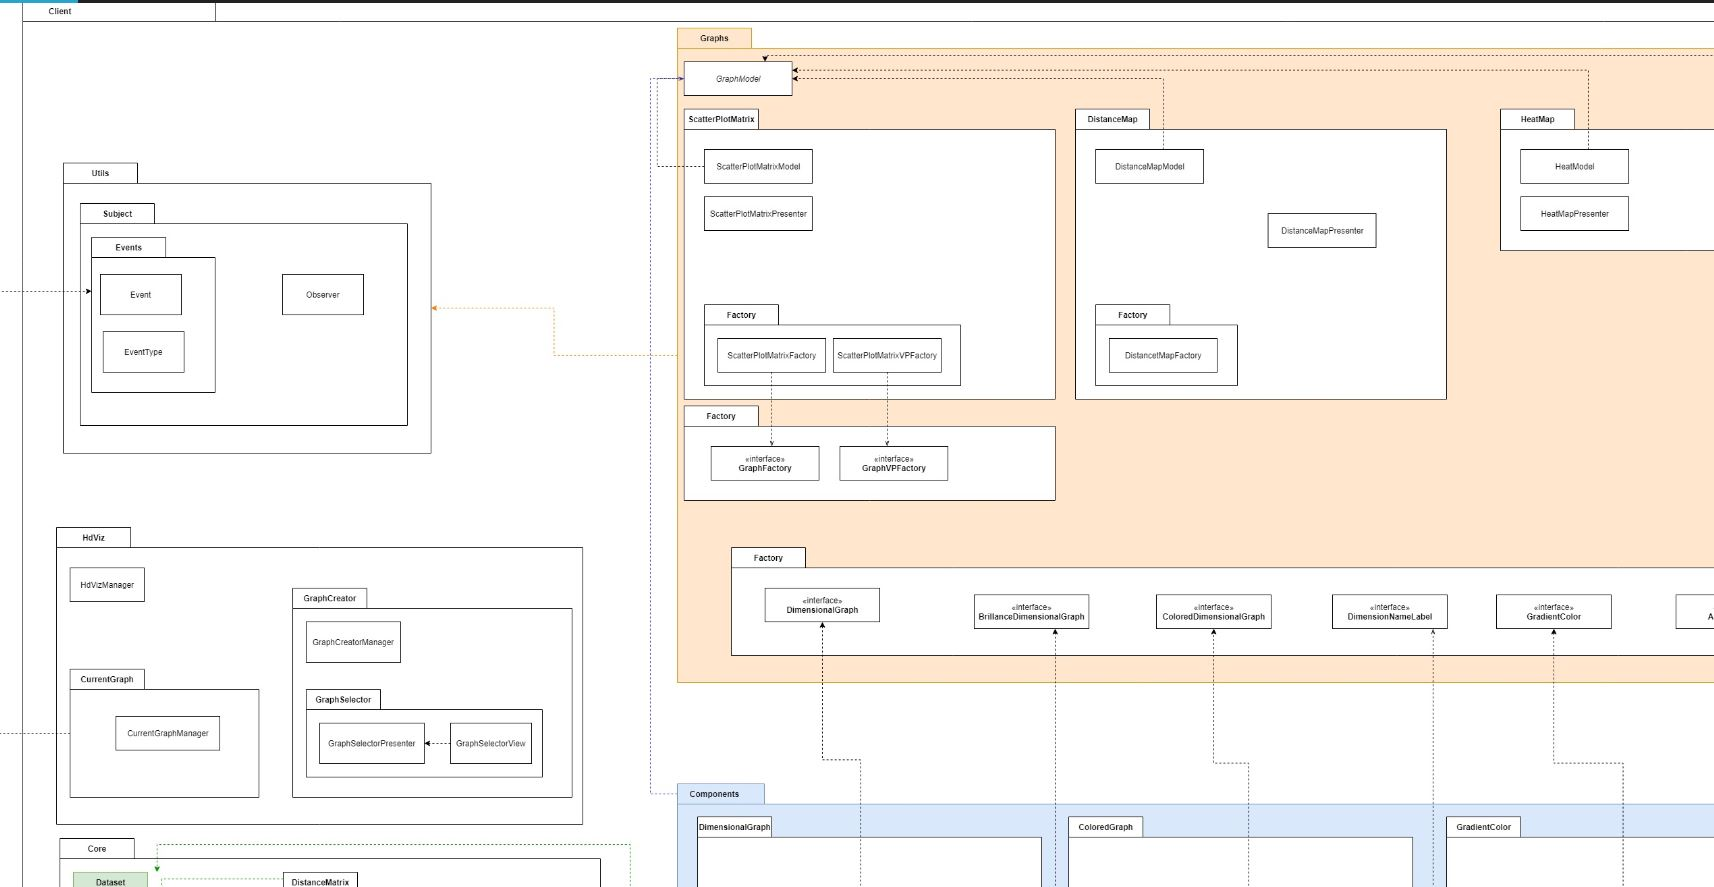
\includegraphics[width=18cm]{img/graph-e-hdviz.jpg}
	\caption{Relazioni tra graph e HD-Viz}
\end{figure}


Ciascun grafico eredita il \emph{GraphModel}; dentro il modello salverà le impostazioni del grafico, ad esempio il gradiente colori, il dataset, i label delle righe ed altro.

\begin{figure}[H]
	\centering
	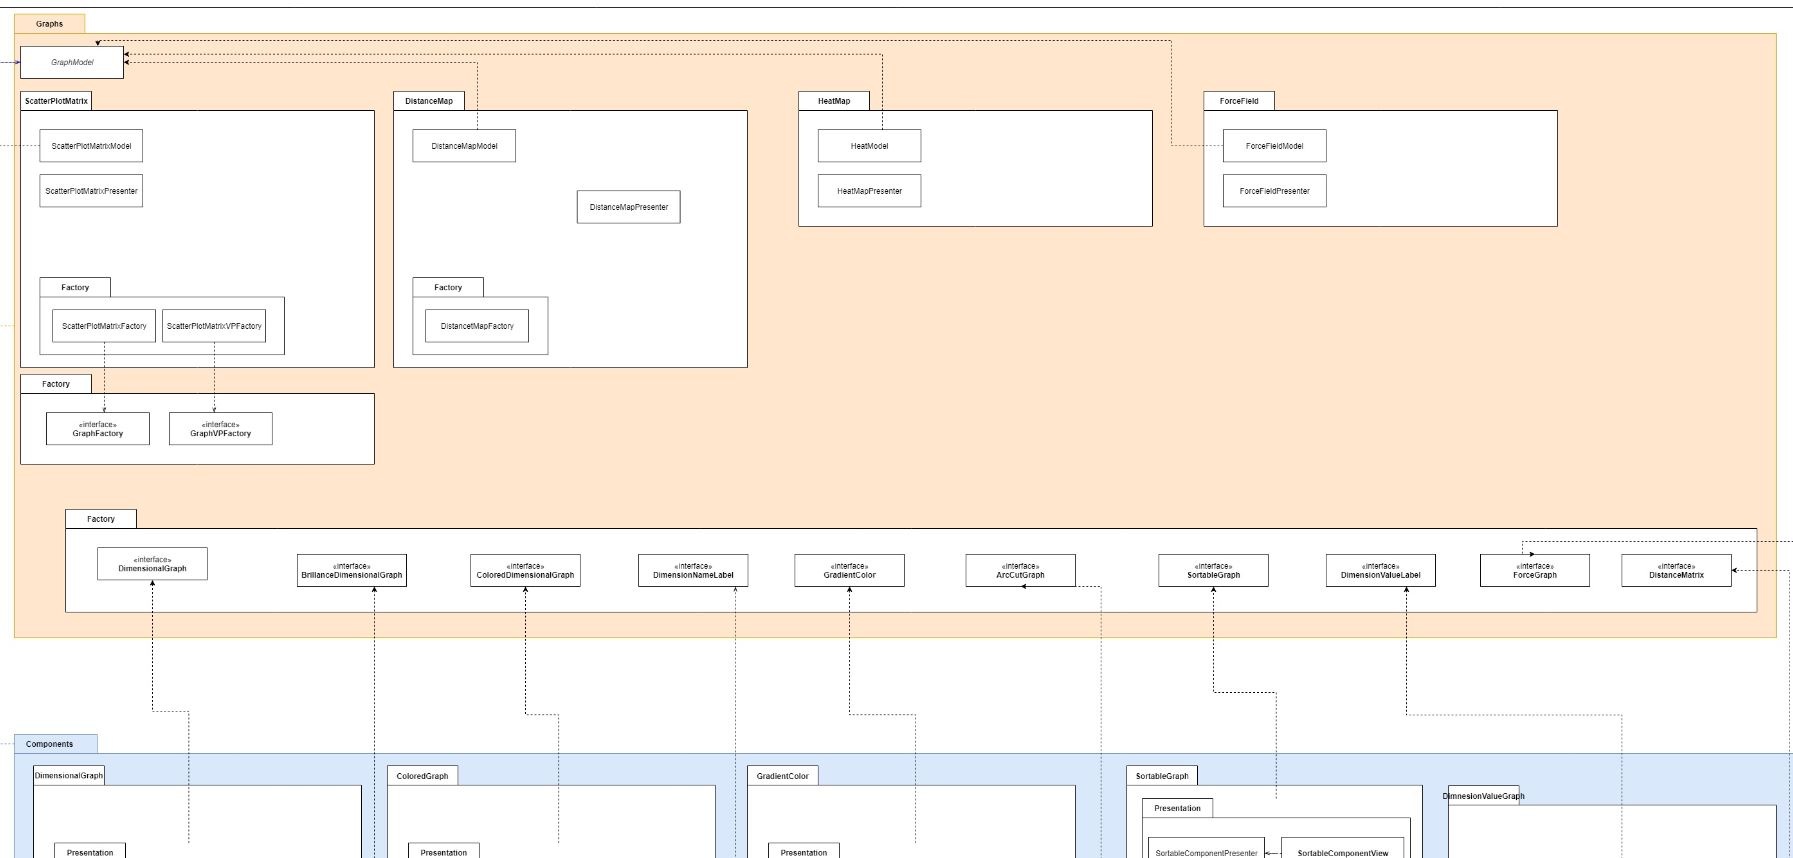
\includegraphics[width=18cm]{img/graphs-e-components.jpg}
	\caption{Relazioni tra graphs e components}
\end{figure}


Collegando il model al presenter, i vari componenti che modificano la visualizzazione notificheranno il presenter; a sua volte modificherà il model, il quale si aggiornerà di conseguenza, 
e notificherà al presenter dei cambiamenti.
Ciò avverrà tramite i metodi update. In particolare al presenter verrà passato l'EventType, ovvero il tipo di evento occorso; in base a ciò si aggiornerà il modello, e quindi la visualizzazione.

\subsubsection{Il Server}

Il lato server dell'applicativo è stato realizzato mediante l'uso del framework \emph{Express}.

Questo si occupa della creazione e gestione di un servizio HTTP. 

\emph{Express} fornisce inoltre un particolare modulo, \emph{Router}, con il quale è possibile definire dei percorsi 
al fine di gestire delle richieste indipendentemente dalla implementazione attuale del server, questo rende possibile
accodareli all'applicativo express finale.

\begin{figure}[H]
	\centering
	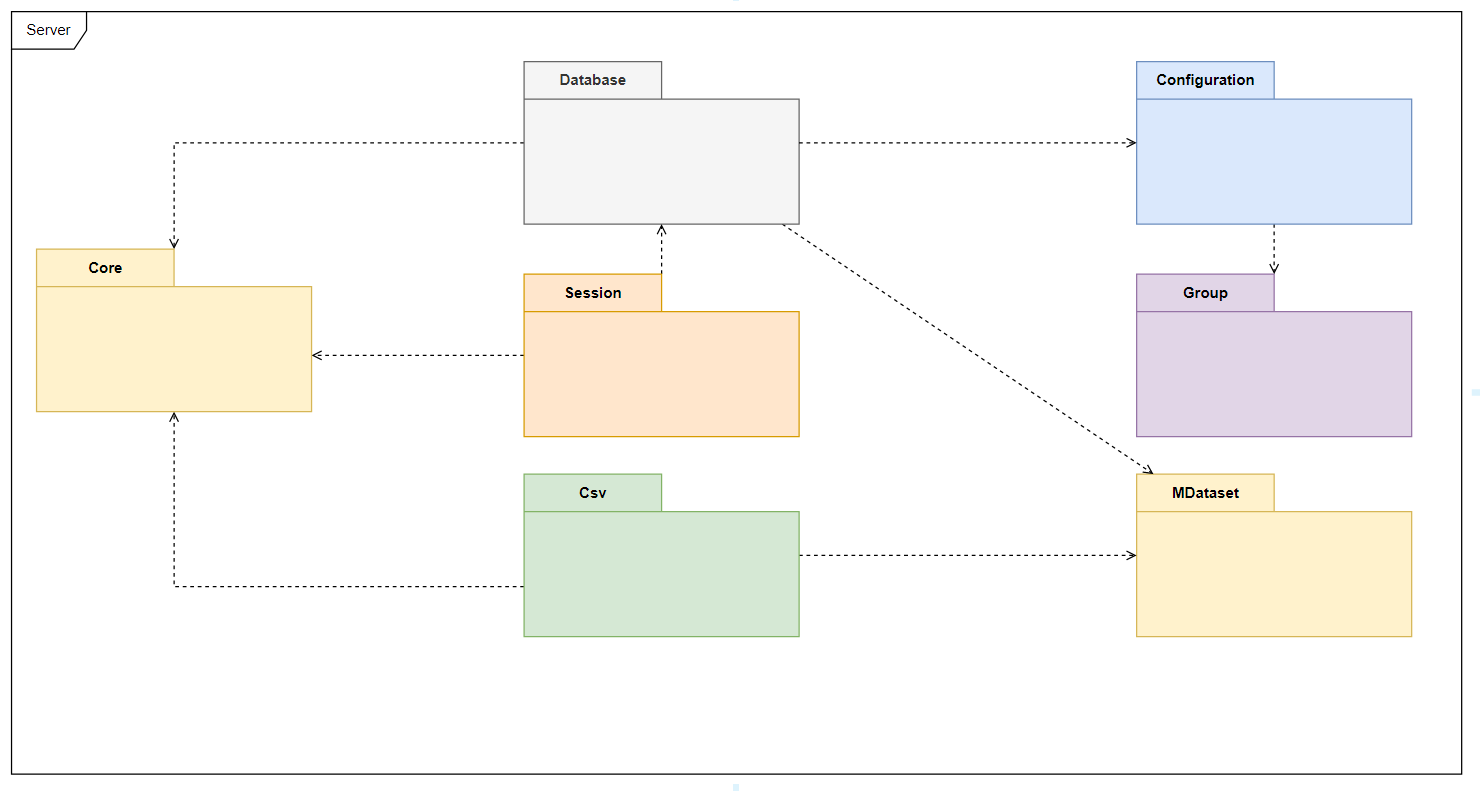
\includegraphics[width=18cm]{img/package-server.png}
	\caption{Diagramma package lato server.}
\end{figure}

\par Presentata la struttura del diagramma di package si riconoscono diversi package.

NB: Al fine di rendere la compresione più chiara vengono riportati frammenti dei diversi diagrammi delle classi, 
quindi verranno eventualmente omesse delle parti laddove non considerate significative.

\begin{itemize}
	
	\item \textbf{Core} Cuore dell'applicativo a lato server, contiene le classi per la gestione del server
	e la definizione di nuovi percorsi da accodare. La classe App definisce il funzionamento del server al quale
	vengono accodate le possibili implemntazioni della classe astratta \emph{Route}, percorsi dinamici,
	e in costruzione i possibili percorsi statici che devono essere resi accessibili. Si occupa inoltre della
	generazione di un ambiento dotato di sessione per il quale ogni percorso implementante \emph{Route} e quindi dotato
	di un Router ha accesso in fase di esecuzione, non essendo tuttavia vincolante per la realizzazione del percorso.
	La creazione della sessione si basa sull'uso delle librerie esterne \emph{express-session} e \emph{memorystore}
	che combinate creano uno store virtuale di oggetti memorizzati per ogni utente che accede al servizio.
		
	\begin{figure}[H]
		\centering
		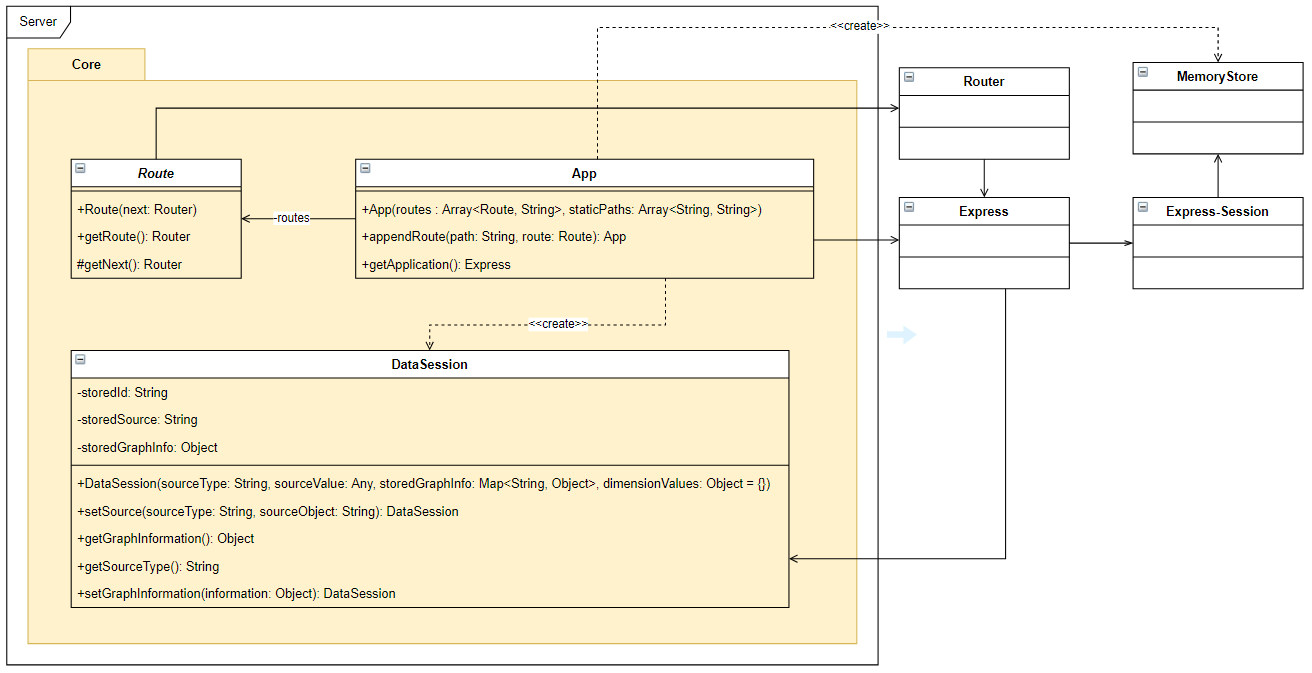
\includegraphics[width=18cm]{img/server-core.png}
		\caption{Classi del package di Core}
	\end{figure}

	\item \textbf{Csv} Package per la gestione delle richieste al server di file csv caricati da client in particolare da \emph{CsvRoute}.
	L'elaborazione, che ricade nella classe \emph{CsvApplication}, avviene mediante l'uso di \emph{fs} per la lettura del file dato in input
	crea una rappresentazione temporanea del dataset al fine di spedire al client un risultato già manipolabile, creando quindi un \emph{MDataset}.
	MDataset non è altro che una rappresentazione dummy del dataset priva di funzionalità.
	
	\begin{figure}[H]
		\centering
		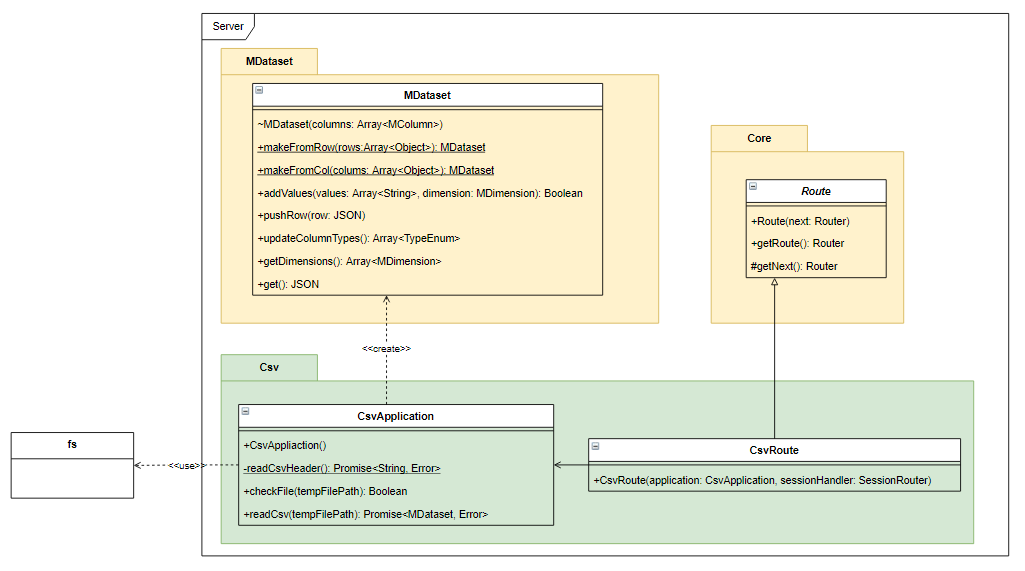
\includegraphics[width=18cm]{img/server-csv.png}
		\caption{Classi del package di Csv}
	\end{figure}


	\item \textbf{Database} Il package per il riperimento dei dati da un database su un dato server.
	Il funzionamento si basa sull'uso di configurazioni che vengono date in costruzione alla classe 
	\emph{RelationalDbApplication} che permettono di eseguire query su un determinato database date le informazioni 
	sfruttando l'ORM Sequelize. Il Dataset costruito dalla query eseguita sul dato server SQL viene poi rispetito al client
	come avviene nel package Csv, la \emph{RelationalDbRoute} infatti, realizzando la classe \emph{Route} è in grado di gestire richieste HTTP e di emetterne.

	\begin{figure}[H]
		\centering
		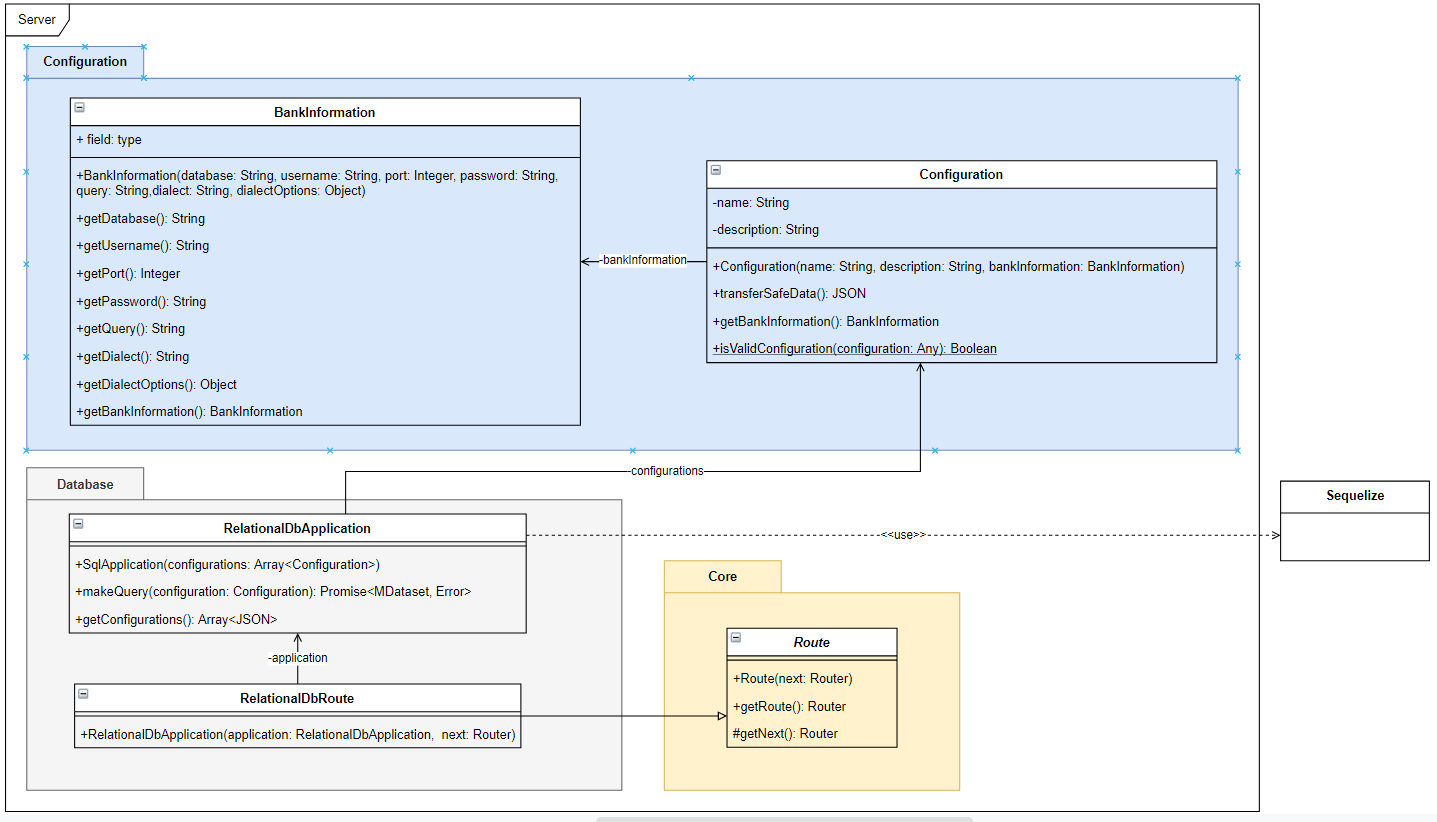
\includegraphics[width=18cm]{img/server-database.png}
		\caption{Classi del package di Database}
	\end{figure}


	\item \textbf{Configuration e Group} Il package di Group contiene delle semplici classi per il controllo di gruppi
	di file con lo stesso nome ma diversa estensione in un determinato percorso, questo si presta al reperimento delle 
	configurazioni per accedere ad un database che sono divise in un file .json e uno .sql, per la query. 
	Infatti il \emph{Configuration Collector} dato un \emph{Group} è in grado di ricostruire configurazioni che 
	come già detto, sono una rappresentazione di tutte le informazioni necessarie per accedere ad una determinata fonte di dati.
	\begin{figure}[H]
		\centering
		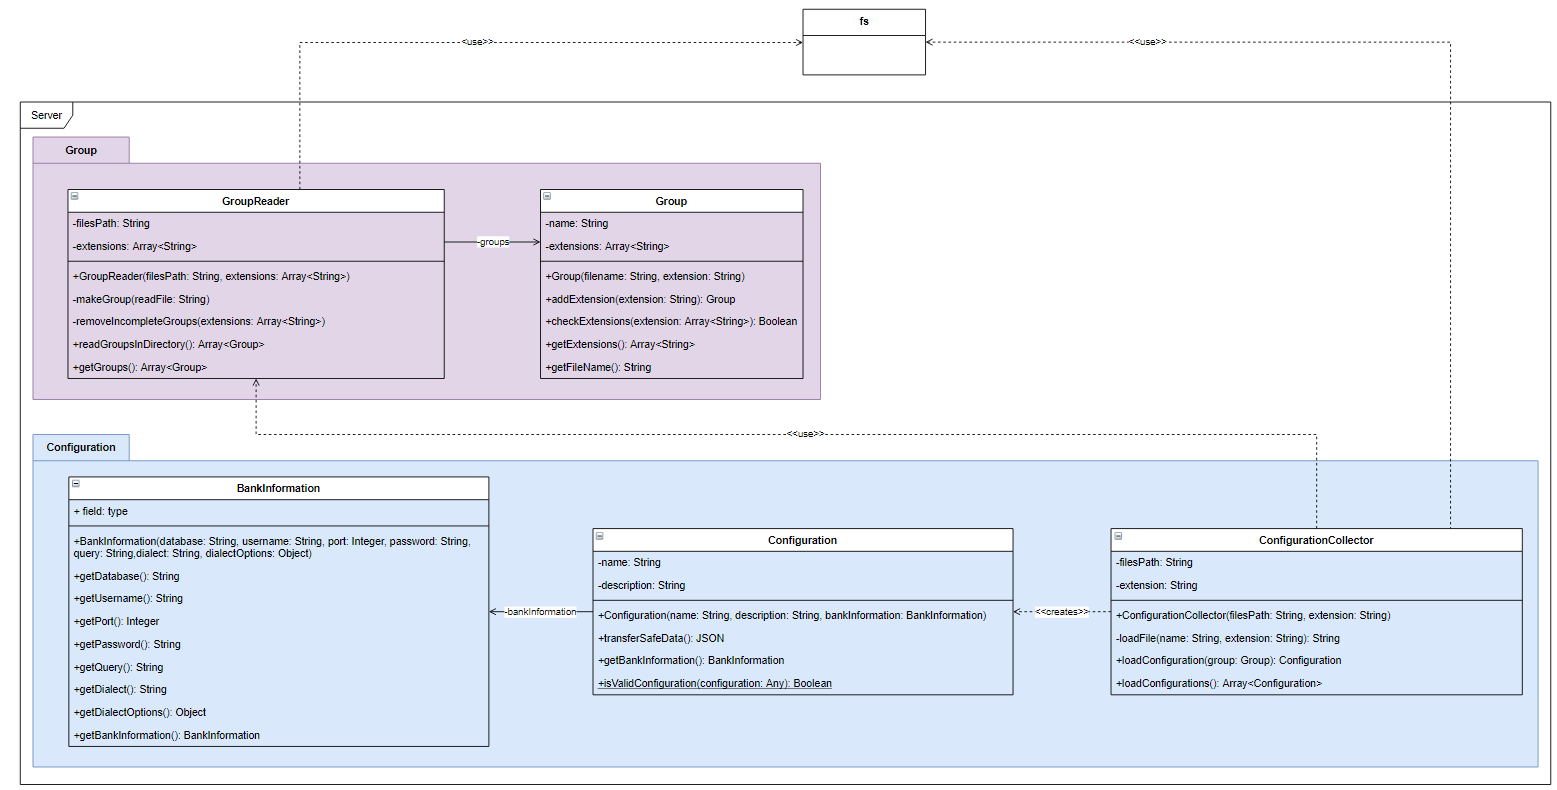
\includegraphics[width=18cm]{img/server-group.png}
		\caption{Classi del package di Configuration e Group}
	\end{figure}

	\item \textbf{MDataset} Package conentente una rappresentazione in versione minimal, priva quindi di funzionalità, del dataset
	che viene calcolato a lato server e spedito al client, in particolare usate dai package \emph{Csv, Database}.

	\item \textbf{Session} Package che contiene la classe per la gestione e il mantenimento della sessione per ogni utente che 
	accede al servizio di HdViz, esso permette di ottenere informazioni sulla propria \emph{DataSession} o di  
	memorizzare delle modifiche avvenute a lato client sulla sessione.

\end{itemize}




Per mantenere i dati coerenti durante l'esecuzione dell'applicativo il server si mette in ascolto  
ad eventuali notifiche che vengono gestite dal \emph{SessionRoute}.

\paragraph{Route e Application} La logica principale del server viene gestita dalla classe \emph{Application},
essa infatti prende una qualsiasi \emph{Route}, classe astratta, e ne gestisce l'aggiunta sul principale
componente di esecuzione di \emph{Express}.


Il lato server è stato realizzato con \emph{Express}, il quale si occuperà di gestire la sessione per collegarsi al server.
SQLApplication si occuperà di caricare la configurazione, che verrà passata ad SQLRoute.\\
Configuration e ConfigurationController si occuperanno di raccogliere le informazioni relative alla connessione con un database, la quale verrà stabilita tramite un file
json dove vi sarà presente la query.\\
MDataset (MinimalDataset) controllerà che il dataset passato sia valido perchè potrebbero esserci oggetti che non possono essere rappresentati. Successivamente
CSVApplication si occuperà di creare un file JSON che contenga i dati letti, se il file è corretto, allora CSVRuoute risponderà positivamente.

\begin{figure}[H]
	\centering
	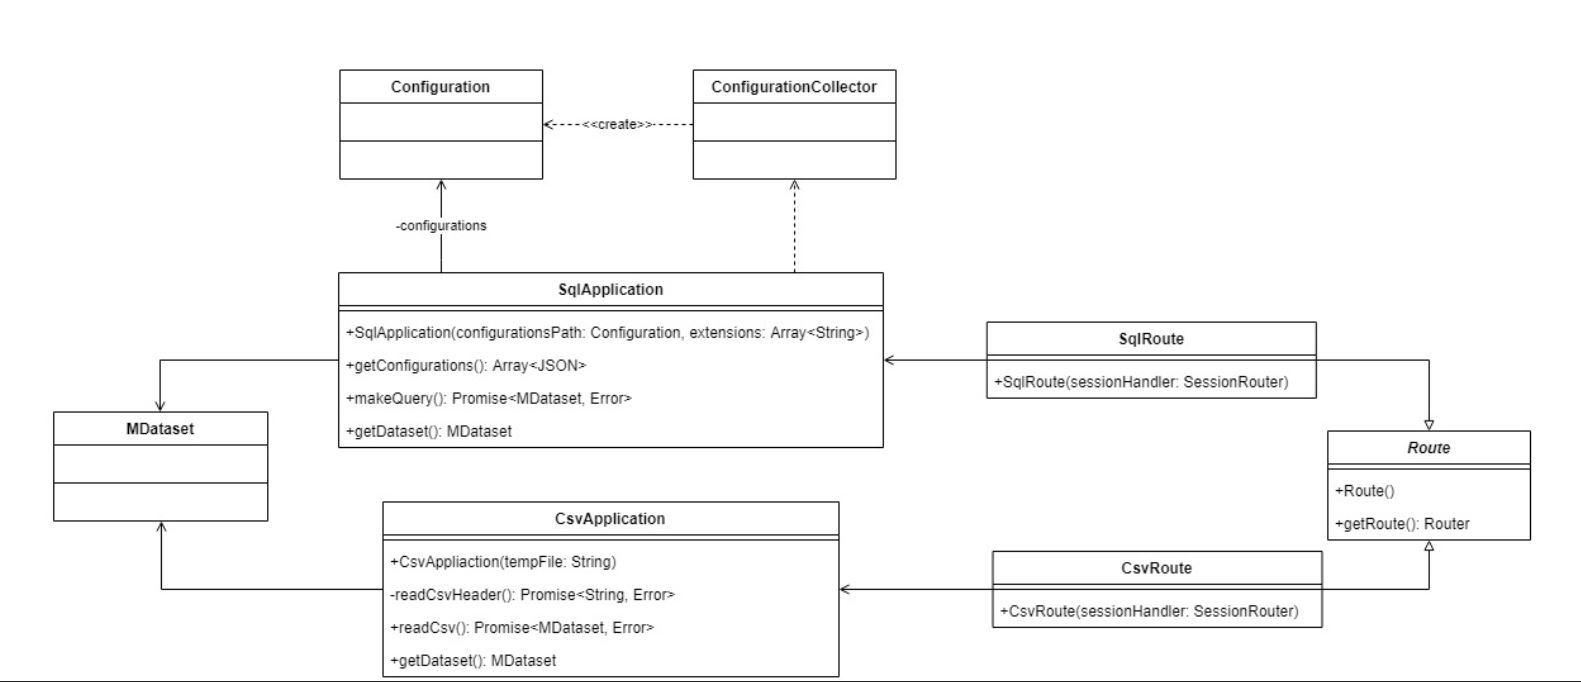
\includegraphics[width=18cm]{img/server.jpg}
	\caption{Server HD-Viz}
\end{figure}

\end{document}